\documentclass[a4paper, 12pt]{article}
\usepackage{fancyhdr}
\usepackage[12pt]{moresize}
\usepackage[pdftex]{graphicx}
\usepackage{epstopdf}
\pagestyle{empty}
\addtolength{\oddsidemargin}{-.875in}
\addtolength{\evensidemargin}{-.875in}
\addtolength{\textwidth}{1.75in}
\addtolength{\topmargin}{-.875in}
\addtolength{\textheight}{1.75in}
\begin{document}
\begin{center}
	{\LARGE {\textbf {MM2090 ASSIGNMENT-4}}}
\end{center}

\section{Student Details}
\textbf {Name} : \textbf{\textit {Bhagat Singh S}}\\
\textbf {Roll No.} : \textbf{\textit {MM20B011}}\\
\textbf {Group} : \textbf{\textit {Group-1}}
\section{The Time Dilation Equation}
\subsection{The Equation}
\begin{equation}
	{\LARGE{\textbf{$t' =\frac{t}{ \sqrt {1 - {\frac{v^2}{c^2}}}}$}}}
	\label{eq:1}
\end{equation}
{\normalsize {Equation \ref{eq:1}  has terms \textbf{t'} ,\textbf{t} , \textbf{v} and \textbf{c}.}}

{\normalsize { Here,}\\
{\normalsize {\textbf{t'} represents the time taken by the moving object}}\\
{\normalsize {\textbf{t} \  represents the time taken by light}}\\
{\normalsize {\textbf{v} \  represents the speed of the moving object}}\\
{\normalsize {\textbf{c} \  represents the speed of light}}
\subsection{Description}

{\small {This theory is derived from the Special Theory of Relativity devised by Albert Einstein.}}
\cite{einstein}

{\small {In physics and relativity, time dilation \cite{Britannica} is the difference in the elapsed time as measured by two clocks. It is either due to a relative velocity between them or to a difference in gravitational potential between their locations.
\begin{figure}[h]
	\centerline{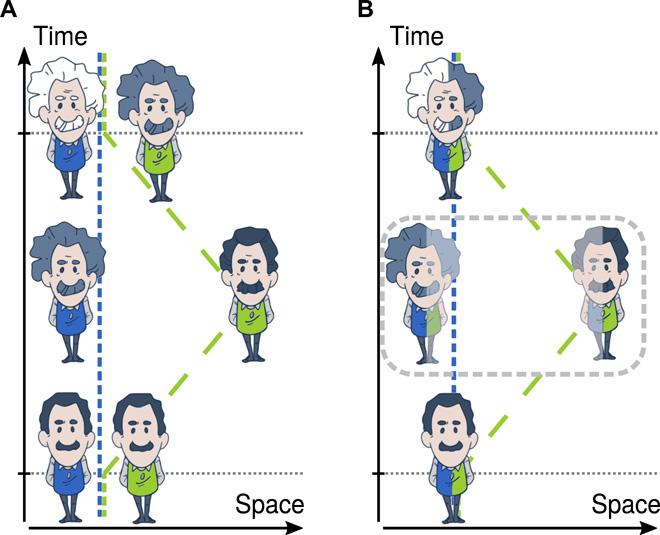
\includegraphics[scale=0.244]{MM20B011}}
	\caption{Twin Paradox}
        \label{fig:1}
\end{figure}

A closely related phenomenon predicted by special relativity is the so-called twin paradox \cite{ScienceAdvances}. Suppose one of two twins carrying a clock departs on a rocket ship from the other twin, an inertial observer, at a certain time, and they rejoin at a later time. In accordance with the time-dilation effect, the elapsed time on the clock of the twin on the rocket ship will be smaller than that of the inertial observer twin—i.e., the non-inertial twin will have aged less than the inertial observer twin when they rejoin.(see Figure \ref{fig:1})
}}

{\small {The time-dilation effect \cite{Wikipedia} predicted by special relativity has been accurately confirmed by observations of the increased lifetime of unstable elementary particles traveling at nearly the speed of light.
}}
\bibliographystyle{IEEEtran}
\bibliography{MM20B011.bib}

\end{document}
